\documentclass{beamer}
\usepackage{listings}
\lstset{
%language=C,
frame=single, 
breaklines=true,
columns=fullflexible
}
\usepackage{blkarray}
\usepackage{subcaption}
\usepackage{url}
\usepackage{tikz}
\usepackage{tkz-euclide} % loads  TikZ and tkz-base
%\usetkzobj{all}
\usetikzlibrary{calc,math}
\usepackage{float}
\newcommand\norm[1]{\left\lVert#1\right\rVert}
\renewcommand{\vec}[1]{\mathbf{#1}}
\usepackage[export]{adjustbox}
\usepackage[utf8]{inputenc}
\usepackage{amsmath}
\usepackage{tikz}
\usepackage{hyperref}
\usepackage{bm}
\hypersetup{
    colorlinks = true,
    linkbordercolor = {white},
    linkcolor={red},
    citecolor={green},
    filecolor={blue},
	menucolor={red},
	runcolor={cyan},
	urlcolor={blue},
	breaklinks=true
}
\usetikzlibrary{automata, positioning}
\usetheme{Boadilla}
\providecommand{\pr}[1]{\ensuremath{\Pr\left(#1\right)}}
\providecommand{\mbf}{\mathbf}
\providecommand{\qfunc}[1]{\ensuremath{Q\left(#1\right)}}
\providecommand{\sbrak}[1]{\ensuremath{{}\left[#1\right]}}
\providecommand{\lsbrak}[1]{\ensuremath{{}\left[#1\right.}}
\providecommand{\rsbrak}[1]{\ensuremath{{}\left.#1\right]}}
\providecommand{\brak}[1]{\ensuremath{\left(#1\right)}}
\providecommand{\lbrak}[1]{\ensuremath{\left(#1\right.}}
\providecommand{\rbrak}[1]{\ensuremath{\left.#1\right)}}
\providecommand{\cbrak}[1]{\ensuremath{\left\{#1\right\}}}
\providecommand{\lcbrak}[1]{\ensuremath{\left\{#1\right.}}
\providecommand{\rcbrak}[1]{\ensuremath{\left.#1\right\}}}
\providecommand{\abs}[1]{\vert#1\vert}

\title{Project Presentation}
\author{Chirag Mehta}
\date{AI20BTECH11006}
\begin{document}

\begin{frame}
\titlepage
\end{frame}
\begin{frame}
\frametitle{A Simple Design of IRS-NOMA Transmission}
\begin{block}{SDMA}
Traditional cellular mobile network systems have no information where the user is located, this wastes a lot of power by sending signals to places where it is not required. Similarly, the antenna at base station recieves signals from all directions including noise. In SDMA, by using smart antenna technology, it differs between the spacial location of mobile units within cell.
\end{block}
\end{frame}
\begin{frame}
\frametitle{SDMA}
\begin{figure}[H]
\centering
\includegraphics[width=.75\linewidth]{figure/SDMA}
\caption{SDMA}
\label{plot:SDMA}
\end{figure}
Image credits: \href{https://slideplayer.com/slide/13883994/}{Source}
\end{frame}

\begin{frame}
\frametitle{A Simple Design of IRS-NOMA Transmission}
\begin{block}{NOMA}
The key idea of NOMA is to use power domain, whereas previous generations used TDMA, CDMA, FDMA. The key advantage of NOMA is that it saves frequency band. SDMA follows Orthogonal Multiple Access, while NOMA is non-orthogonal. However, SDMA is better than NOMA if the user channel vectors are orthogonal to each other, while if the are in same direction NOMA is better. \\
N is the number of reflecting surfaces in IRS, we have two arbitrary constants $P$, $Q$ such that $PQ=N$

\end{block}
\end{frame}
\begin{frame}
\frametitle{IRS-NOMA}
\begin{figure}[H]
\centering
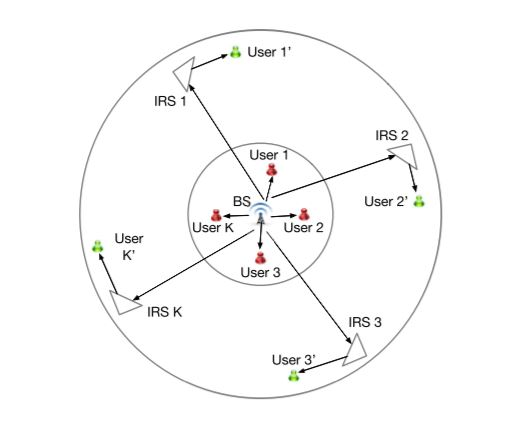
\includegraphics[width=.75\linewidth]{figure/irs-noma}
\caption{IRS-NOMA}
\label{plot:irs-noma}
\end{figure}
\end{frame}

\begin{frame}
\frametitle{System Model}
We'll assume that on each beak $\boldsymbol{w_k}$ one additional user denoted by $k'$ is served.
The base station broadcasts
\begin{align}
y_{k'}=\displaystyle\sum_{k=1}^K \boldsymbol{w_k}\brak{\alpha_1 s_k+\alpha_2 s_{k'}}
\end{align}
SINR (Signal to Inteference and noise ratio) is given as
\begin{align}
\text{\textbf{SINR}}_{k'}=\frac{\abs{\boldsymbol{\theta}_K^H \boldsymbol{D}_{k'}\boldsymbol{h}_k}^2\alpha_2^2}{\abs{\boldsymbol{\theta}_K^H \boldsymbol{D}_{k'}\boldsymbol{h}_k}^2\alpha_1^2+\sum_{i=1\,,i\neq k}^{K}\abs{\boldsymbol{\theta}_K^H \boldsymbol{D}_{k'}\boldsymbol{h}_i}^2+\frac{1}{\rho}}
\end{align}
where $\rho$ represents signal to noise ratio (SNR), $\boldsymbol{\Theta}_k$ is a diagonal matrix, and each of its main diagonal elements is denoted by $\beta_{k,\,i}e^{-j\theta_{k,\, i}}$, where $\theta_{k,\, i}$ denotes the reflection phase shift and $\beta_{k,\, i}$ denotes the amplitude reflection coefficient.
\end{frame}
\begin{frame}
\frametitle{Outage probability}
\begin{block}{Outage probability}
Outage probability is defined as the point at which the receiver power value falls below the threshold (where the power value relates to the minimum signal to noise ratio (SNR) within a cellular), one can say that the receiver is out of the range of BS in cellular communications.
\end{block}

\end{frame}
\begin{frame}
\frametitle{Outage Probability}
Lets first discuss about single user case, $K=1$\\
The probability density function of outage at $k'$ is given by
\begin{align}
f_{Q\abs{\boldsymbol{v}_P^H \boldsymbol{D}_{k'}\boldsymbol{h}_k}^2}(x)=\frac{2x^{\frac{Q-1}{2}}}{\Gamma(Q)} K_{Q-1}\brak{2\sqrt{x}}
\end{align}
Now to find the probability, we'll integrate the pdf
\begin{align}
\pr{k',\,p}&=\int\limits_{0}^{\xi} f_{Q\abs{\boldsymbol{v}_P^H \boldsymbol{D}_{k'}\boldsymbol{h}_k}^2}(x)\,dx\\
&=\frac{2}{\Gamma(Q)}\int\limits_{0}^{\xi}x^{\frac{Q-1}{2}}K_{Q-1}\brak{2\sqrt{x}}\,dx\\
&=\frac{1}{\Gamma(Q)}\xi^{\frac{Q+1}{2}}\brak{\xi^{-\frac{Q+1}{2}}\Gamma(Q)-2\xi^{-\frac{1}{2}}K_{Q}\brak{2\xi^\frac{1}{2}}}
\end{align}
where $\xi=\frac{Q\epsilon_{k'}}{\rho(\alpha_2^2-\alpha_1^2\epsilon_{k'})}$
\end{frame}

\begin{frame}
\frametitle{Modified Bessel function}
\begin{block}{Modified Bessel function}
The modified Bessel function $K_\alpha(x)$ is defined as 
\begin{align}
K_\alpha(x)=\frac{\pi}{2}\frac{I_{-\alpha}(x)-I_\alpha(x)}{\sin{\alpha\pi}}
\end{align}
where $I_\alpha(x)$ is defined as
\begin{align}
I_\alpha(x)=\displaystyle\sum_{m=0}^{\infty}\frac{1}{m!\Gamma(m+\alpha+1)}\brak{\frac{x}{2}}^{2m+\alpha}
\end{align} 
\end{block}
\end{frame}

\begin{frame}
\frametitle{Approximation of outage probability}
The outage probability at $k'$ is given by
\begin{align}
\pr{k'}=\frac{\xi^{\frac{P(Q+1)}{2}}}{(\Gamma(Q))^P}\brak{\xi^{-\frac{Q+1}{2}}\Gamma(Q)-2\xi^{-\frac{1}{2}}K_{Q}\brak{2\xi^\frac{1}{2}}}^P\label{eq:prob_1}
\end{align}
The bessel function can be approximated as
\begin{align}
K_n(z)\approx\frac{1}{2}\brak{\frac{(n-1)!}{\brak{\frac{z}{2}}^n}-\frac{(n-2)!}{\brak{\frac{z}{2}}^{n-2}}}\label{eq:bessel_approx_1}
\end{align}
This approximation is valid for $z\to 0,\, n\geq 2$, for $n=1$ the following approximation is correct.
\begin{align}
K_1(z)\approx \frac{1}{2} \frac{1}{\brak{\frac{z}{2}}}+\brak{\frac{z}{2}}\ln\brak{\frac{z}{2}}\label{eq:bessel_approx_2}
\end{align}
\end{frame}

\begin{frame}
\frametitle{Approximation of outage probability contd.}
Using \eqref{eq:prob_1} and \eqref{eq:bessel_approx_1}, this is the case where $Q\geq 2$
\begin{align}
\pr{k'}&\approx \frac{1}{(\Gamma(Q))^P}\brak{\Gamma(Q)-\xi^\frac{Q}{2}\brak{\frac{(Q-1)!}{\xi^\frac{Q}{2}}-\frac{(Q-2)!}{\xi^\frac{Q-2}{2}}}}^P\\
&\approx \frac{\xi^P}{(Q-1)^P}
\end{align}
Using \eqref{eq:prob_1} and \eqref{eq:bessel_approx_2}
\begin{align}
\pr{k'}&\approx \brak{1-\xi\brak{\frac{1}{\xi^\frac{1}{2}}+\xi^\frac{1}{2}\ln\brak{\xi}}}^P\\
&\approx \xi^N\brak{-\ln\brak{\xi}}^N
\end{align}

\end{frame}

\begin{frame}
\frametitle{Diversity Gain}
\begin{block}{Diversity Gain}
Diversity gain is the increase in signal-to-interference ratio due to some diversity scheme, or how much the transmission power can be reduced when a diversity scheme is introduced, without a performance loss. Diversity gain is usually expressed in decibels, and sometimes as a power ratio.
\end{block}
\end{frame}

\begin{frame}
\frametitle{Diversity gain}
\begin{align}
\pr{k'}\approx
\begin{cases}
\xi^N\brak{-\ln\brak{\xi}}^N& Q=1\\
\frac{\xi^P}{(Q-1)^P} & Q\geq 2
\end{cases}
\end{align}
The diversity gain is given as
\begin{enumerate}
\item For $Q=1$
\begin{align}
-\lim_{\rho\to\infty}\frac{\log\brak{\pr{k'}}}{\log\brak{\rho}}=\lim_{\xi\to 0}\frac{\log\brak{\xi^N(-\ln(\xi))^N}}{\log\brak{\xi}}=N
\end{align}
\item For $Q\geq 2$\\
It is very easy to obtain that diversity gain is $P$
\end{enumerate}
Thus, the choice $Q=1$ is optimal to IRS-NOMA with on-off control.
\end{frame}

\begin{frame}
\frametitle{Single user case simulation}
The simulation for single user case is given below.
\begin{figure}[H]
\centering
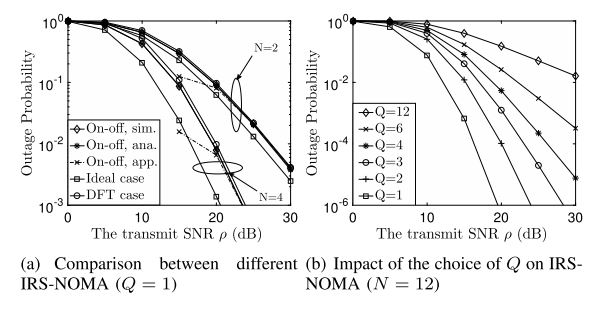
\includegraphics[width=.75\linewidth]{figure/snr_q}
\caption{Impact of IRS-NOMA on the downlink outage probability for the single-user case ($K=1$). $M=4$. $R_k'=2$ bits per channel use (BPCU)}
\label{fig:fig3}
\end{figure}
\end{frame}


\begin{frame}
\frametitle{Multiuser case simulation}
For multi-user case, we will restrain ourselves to only $Q=1$ case because simulations show it is the optimal one.
\begin{figure}[H]
\centering
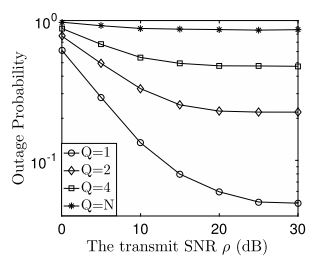
\includegraphics[width=.65\linewidth]{figure/multi_q}
\caption{Effects of Q}
\label{fig:4}
\end{figure}

\end{frame}
\begin{frame}
\frametitle{Outage probability in multiuser case}
For multiuser case, the outage probability is given by
\begin{align}
\pr{k'}\approx\brak{1-\frac{1}{\brak{1+\frac{\epsilon_{k'}}{\tau}}^{K-1}}}^N
\end{align}
The outage probability does not go to zero by simply increasing the transmission power. However, the outage probability can be reduced by increasing $N$.
\end{frame}

\begin{frame}
\frametitle{Conclusion}
In this research paper, it was proposed to serve a near user and a cell edge user on a single orthogonal beam if number of users $K<M$, in typical SDMA, it would require $2K$ separate beams. it was assumed that there is no direct link between cell edge user and base station. It can be noted that the proposed scheme can be extended to the case where there is a direct link between cell edge user and base station.
\end{frame}
\end{document}